\begin{slide}
\pagestyle{headings}
\sf 
\header{Fit of a constant}
%\begin{center}
\vspace*{2mm}
\Large 
Example: Averaging of $n$ different measurements 
$a_i \pm \sigma_i$ of an observable $a$ (e.g. $a = \alpha_s(m_Z)$)
\[ \chi^2 = \Sigma_i^n \frac{ (a_i - a)^2}{\sigma_i^2} \]
``Idiot example'' of one single measurement $a_1 \pm \sigma_1$:
\[ \chi^2 = \frac{ (a_1 - a)^2}{\sigma_1^2} \]
\[Min. \chi^2: \quad \frac{d \chi^2}{da} = 0 \; 
\rightarrow \; \mbox{Estimated value}\quad
\hat{a} = a_1; \; \sigma_{\hat{a}} = \sigma_1 \]
%
%\end{center}
\end{slide}
%
%
%
%
\begin{slide}
\pagestyle{headings}
\sf 
\header{Fit of a constant {\em (single measurement)}}
\Large 
Probability density $p$ for true value of $a$ ({\em inverse probability}):
\begin{figure}[h]
\unitlength1cm
  \begin{picture}(8,9.)
%    \put(0.,0.){\epsfig{file=feynman/chisqp1.ps,width=8.cm}}
    \put(0.,4){\epsfig{file=feynman/gauss1.ps,width=5.3cm}}
    \put(0.5,-0.6){\epsfig{file=feynman/chisqp1.ps,width=4.8cm}}
\put(1.2,8.2){\large 
$ \pmb{p \sim
%\frac{1}{\sqrt{2\pi}\sigma_{\hat{a}}} \cdot 
e^{- \frac{(a - \hat{a})^2}{2\sigma_{\hat{a}}^2}} 
= e^{-\chi^2/2} 
}
$
}
%
\put(5.8,8.3){
\begin{minipage}[t]{6.5cm}
\Large $\rightarrow$
Important general relation:\\[2mm]
$\displaystyle \sigma_{\hat{a}} = 
\left[ -\frac{d^2\chi^2}{da^2}_{|a=\hat{a}} \right]^{-1/2}
$
\end{minipage}
}
\put(6.0,2.7){
\begin{minipage}[t]{6.5cm}
\Large $\rightarrow$
Important general relation:\\[2mm]
\Large $\chi^2(\hat{a}+\sigma_{\hat{a}}) = 1$
\end{minipage}
}
\end{picture}
\end{figure}
\end{slide}
